\documentclass[aspectratio=169,UTF8,zihao=-4]{ctexbeamer}

\usetheme{Madrid}
\usecolortheme{default}
\setbeamertemplate{navigation symbols}{}
\setbeamertemplate{headline}{}
\setbeamertemplate{frametitle}{}
\setbeamertemplate{footline}[frame number]

\usepackage{amsmath}
\usepackage{booktabs}
\usepackage{array}
\usepackage{tikz}
\usetikzlibrary{arrows.meta,positioning}

\title{范文2第1次提交\\网站美学与消费者购物价值}
\author{王鲲淏-22307100011}
\date{Social Research}

\newcommand{\bigidea}[1]{
  \begin{center}
    \vspace{0.8em}
    {\LARGE \bfseries #1}
    \vspace{0.6em}
  \end{center}
}

\newcommand{\sectionpageframe}[1]{
  \begin{frame}[plain]
    \begin{center}
      \vfill
      {\Huge \bfseries #1}
      \vfill
    \end{center}
  \end{frame}
}

\begin{document}

\begin{frame}[plain]
  \titlepage
\end{frame}

\sectionpageframe{理论基础}

\begin{frame}
  \bigidea{本文的理论}
  \begin{itemize}
    \item \Large 网站美学二维框架：Classical Aesthetics 与 Expressive Aesthetics。
    \item \Large 消费者购物价值理论：购物价值可分为 utilitarian 与 hedonic 两部分。
    \item \Large 任务匹配逻辑：不同产品类型会改变用户对网站美学线索的重视程度。
    \item \Large 因而本文不是只研究“美不美”，而是研究“美学如何转化为购物价值”。
  \end{itemize}
\end{frame}

\sectionpageframe{变量与定义}

\begin{frame}
  \bigidea{自变量与因变量}
  \small
  \begin{tabular}{p{3.0cm}p{7.0cm}}
    \toprule
    变量 & 定义 \\
    \midrule
    Expressive Aesthetics & 网站在原创性、视觉吸引力、丰富性与表现力上的美学感知。 \\
    Classical Aesthetics & 网站在秩序性、清晰性、和谐性与布局直观性上的美学感知。 \\
    Shopping Enjoyment & 用户在浏览和购物过程中感到有趣、愉快、兴奋的程度。 \\
    Shopping Process Value & 网站是否提升购物效率、效果与生产率的感知。 \\
    Product Type & 产品类型，分为 hedonic product 与 utilitarian product。 \\
    \bottomrule
  \end{tabular}
\end{frame}

\sectionpageframe{自变量操纵}

\begin{frame}
  \bigidea{实验如何操纵自变量}
  \begin{itemize}
    \item \Large Expressive aesthetics 通过颜色方案操纵。
    \item \Large 研究者改变背景、文字和边框的颜色组合，形成高/低 expressive 条件。
    \item \Large Classical aesthetics 通过功能布局操纵。
    \item \Large 研究者调整首页、列表页和详情页的栏目位置，使布局更符合或偏离常规网站结构。
    \item \Large Product type 通过购物对象操纵：数码相机、笔记本代表 utilitarian；香水、鲜花代表 hedonic。
  \end{itemize}
\end{frame}

\sectionpageframe{实验流程}

\begin{frame}
  \bigidea{实验流程}
  \begin{enumerate}
    \item \Large 先做小规模产品筛选测试，从 8 类在线产品中选出享乐型与功利型产品。
    \item \Large 再做量表预测试：44 名学生完成模拟购物任务，用 EFA 检验量表结构。
    \item \Large 正式实验采用 $2 \times 2 \times 2$ 设计，173 名学生被随机分配到 8 个条件。
    \item \Large 每位参与者完成两次模拟购物，共得到 346 个观测值。
  \end{enumerate}
\end{frame}

\sectionpageframe{测量方式}

\begin{frame}
  \bigidea{自变量和因变量如何测量}
  \small
  \begin{itemize}
    \item Expressive aesthetics：例如“网站看起来有吸引力”“我喜欢这个网站的外观与感觉”。
    \item Classical aesthetics：例如“网站设计是和谐的”“网站布局直观”“元素组织有逻辑”。
    \item Shopping enjoyment：例如“本次访问很有趣/愉快/令人兴奋”。
    \item Shopping process value：例如“该网站提升了我的购物表现、效率和有效性”。
    \item 正式实验中，作者使用 CFA 检验四个多题项构念，并报告 Cronbach's alpha、AVE 等指标。
  \end{itemize}
\end{frame}

\sectionpageframe{研究模型}

\begin{frame}
  \bigidea{研究模型图}
  \centering
  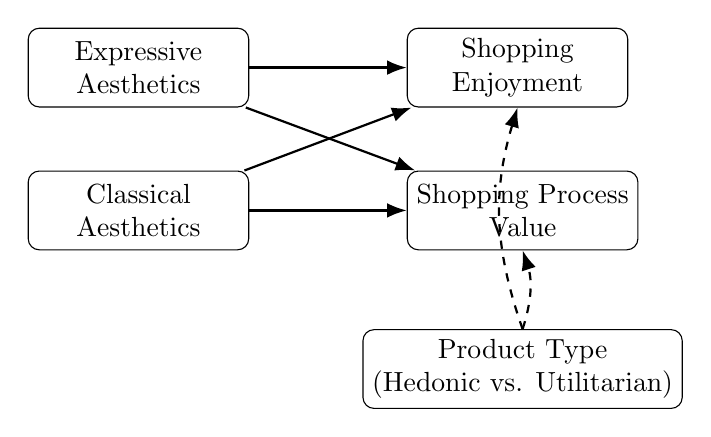
\begin{tikzpicture}[
    node distance=0.8cm and 1.1cm,
    box/.style={draw, rounded corners, align=center, minimum width=2.8cm, minimum height=1.0cm},
    arr/.style={-{Latex[length=2.5mm]}, thick}
  ]
    \node[box] (ea) {Expressive\\Aesthetics};
    \node[box, below=of ea] (ca) {Classical\\Aesthetics};
    \node[box, right=2.0cm of ea] (enj) {Shopping\\Enjoyment};
    \node[box, right=2.0cm of ca] (pv) {Shopping Process\\Value};
    \node[box, below=1.0cm of pv] (pt) {Product Type\\(Hedonic vs. Utilitarian)};

    \draw[arr] (ea) -- (enj);
    \draw[arr] (ea) -- (pv);
    \draw[arr] (ca) -- (enj);
    \draw[arr] (ca) -- (pv);
    \draw[arr, dashed] (pt.north) to[bend left=18] (enj.south);
    \draw[arr, dashed] (pt.north) to[bend right=18] (pv.south);
  \end{tikzpicture}
\end{frame}

\begin{frame}
  \bigidea{如果老师问“有没有多个实验”}
  \begin{itemize}
    \item \Large 本文主体不是多个独立实验串联，而是一个完整的实验研究流程。
    \item \Large 但可以区分为三个阶段：产品筛选测试、量表预测试、正式实验。
    \item \Large 这三个阶段的任务不同：选材料、验量表、检验假设。
  \end{itemize}
\end{frame}

\end{document}
